% PathoFluor-At slide deck. Numbers come from ../manuscript/numbers.tex (scripts/07_numbers.py);
% figures from ../figures (scripts/08_figures.py). Build: make (in this folder).
\documentclass[aspectratio=169,10pt]{beamer}
\usetheme{Boadilla}
\usecolortheme{default}
\usepackage[utf8]{inputenc}
\usepackage[T1]{fontenc}
\usepackage{graphicx}
\usepackage{xcolor}
\graphicspath{{../figures/}}
% Generated by scripts/07_numbers.py from tables/ and metadata/. Do not edit by hand.
\newcommand{\nFiles}{7,752}
\newcommand{\nCubes}{400}
\newcommand{\nCubesA}{216}
\newcommand{\nCubesB}{168}
\newcommand{\nRoiFiles}{5,842}
\newcommand{\nRoiUnique}{2,486}
\newcommand{\nRoiA}{1,982}
\newcommand{\nRoiB}{504}
\newcommand{\rawGB}{396}
\newcommand{\rawFzero}{2,588}
\newcommand{\rawFone}{2,044}
\newcommand{\rawDropPct}{21}
\newcommand{\cpsDiffPct}{4}
\newcommand{\satHzeroMaxPct}{13}
\newcommand{\satHzeroMedPct}{0.1}
\newcommand{\pathFwhmOneSD}{2.07}
\newcommand{\pathFwhmOnenm}{1.40}
\newcommand{\pathFwhmOneq}{0.018}
\newcommand{\pathFwhmTwoSD}{2.39}
\newcommand{\pathFwhmTwonm}{1.76}
\newcommand{\pathFwhmTwoq}{6.8\times10^{-4}}
\newcommand{\pathSwTwoSD}{1.77}
\newcommand{\pathSwTwoq}{0.018}
\newcommand{\pathFwhmThreenm}{1.02}
\newcommand{\pathFwhmThreeq}{0.005}
\newcommand{\pathSwThreeSD}{2.03}
\newcommand{\pathSwThreeq}{6.9\times10^{-4}}
\newcommand{\pathFwhmTwentyFournm}{3.35}
\newcommand{\pathFwhmTwentyFourq}{0.005}
\newcommand{\pathSwTwentyFourSD}{2.46}
\newcommand{\pathSwTwentyFourq}{4.3\times10^{-5}}
\newcommand{\cmlFourSwSD}{-1.74}
\newcommand{\cmlFourSwq}{0.036}
\newcommand{\flgFwhmThreeSD}{2.18}
\newcommand{\flgFwhmThreeq}{0.005}
\newcommand{\nBaselineTests}{270}
\newcommand{\nBaselineSig}{13}
\newcommand{\hzeroFlgFwhmSD}{-1.29}
\newcommand{\hzeroFlgFwhmq}{5.5\times10^{-5}}
\newcommand{\setBinterSD}{1.78}
\newcommand{\setBinterq}{0.026}
\newcommand{\setBinterN}{4}
\newcommand{\aucPathOne}{1.00}
\newcommand{\pPathOne}{0.029}
\newcommand{\aucPathTwo}{1.00}
\newcommand{\pPathTwo}{0.029}
\newcommand{\aucPathTwentyFour}{1.00}
\newcommand{\pPathTwentyFour}{0.029}
\newcommand{\aucPathThree}{0.75}
\newcommand{\pPathThree}{0.143}
\newcommand{\aucPlaceboFlg}{1.00}
\newcommand{\pPlaceboFlg}{0.029}
\newcommand{\aucPlaceboPath}{0.81}
\newcommand{\aucFlgEarlyMin}{0.89}
\newcommand{\aucFlgEarlyMax}{1.00}
\newcommand{\pFlgEarlyMin}{0.10}
\newcommand{\nPermFlgBase}{20}
\newcommand{\specFlgColO}{0.18}
\newcommand{\specFlgFlsSeventeen}{0.36}
\newcommand{\specFlgFlsOneOhOne}{0.24}
\newcommand{\nUseSubset}{1,358}
\newcommand{\nCopyFiles}{16}
\newcommand{\nOffsetRoi}{83}
\newcommand{\offsetMedian}{109}
\newcommand{\offsetCleanMedian}{0.1}
\newcommand{\nKeyConflict}{12}
\newcommand{\nTagValues}{25}

\newcommand{\pending}[1]{\textcolor{red}{[PENDING: #1]}}
\setbeamertemplate{navigation symbols}{}

\title[PathoFluor-At]{Fluorescence hyperspectral signatures of \textit{Pseudomonas} challenge
and flg22 in \textit{Arabidopsis}}
\subtitle{A FAIR reanalysis of the 2016 UW-Madison experiment}
\author[Barker et al.]{Richard J. Barker \textit{et al.}}
\date{\pending{date / venue}}

\begin{document}

\begin{frame}
  \titlepage
\end{frame}

\begin{frame}{The question}
  \begin{itemize}
    \item Can we \textbf{see} a plant responding to bacteria before symptoms appear?
    \item Plants perceive flagellin (flg22) through the receptor \textbf{FLS2}; \textit{fls2}
          mutants cannot.
    \item \textbf{CML24} (TCH2) is a Ca$^{2+}$ sensor; \textit{cml24-4} is impaired in
          pattern-induced NO signalling.
    \item Chlorophyll fluorescence changes with photosynthesis and chlorophyll content, so a
          \textbf{whole emission spectrum per pixel} might carry an early signature.
  \end{itemize}
  \vfill
  \textbf{Key control:} a genuine flg22 \emph{perception} signature must vanish in \textit{fls2}.
\end{frame}

\begin{frame}{The 2016 experiment}
  \begin{columns}[T]
    \column{0.55\textwidth}
    \begin{itemize}
      \item MacroPhor fluorescence hyperspectral imager (Middleton Spectral Vision), Gilroy Lab
      \item 488\,nm excitation, 500--800\,nm emission, 324 bands
      \item 5 genotypes per plate: Col-0, \textit{fls2-17}, \textit{fls2-101},
            \textit{cml24-2}, \textit{cml24-4}
      \item Mock, flg22 or \textit{P.~syringae}; 4 plates each
      \item Imaged before treatment, then 1, 2, 3, 24 and 48\,h
      \item Independent replicate (Nov 2016, 405\,nm excitation)
    \end{itemize}
    \column{0.42\textwidth}
    \begin{block}{Recovered from the drive}
      \nFiles{} files, \rawGB{}\,GB\\
      \nCubes{} image cubes\\
      \nRoiUnique{} unique hand-drawn seedling spectra\\
      every file name parsed, every cube hashed
    \end{block}
  \end{columns}
\end{frame}

\begin{frame}{Data problem 1: exposure time changed between timepoints}
  \centering
  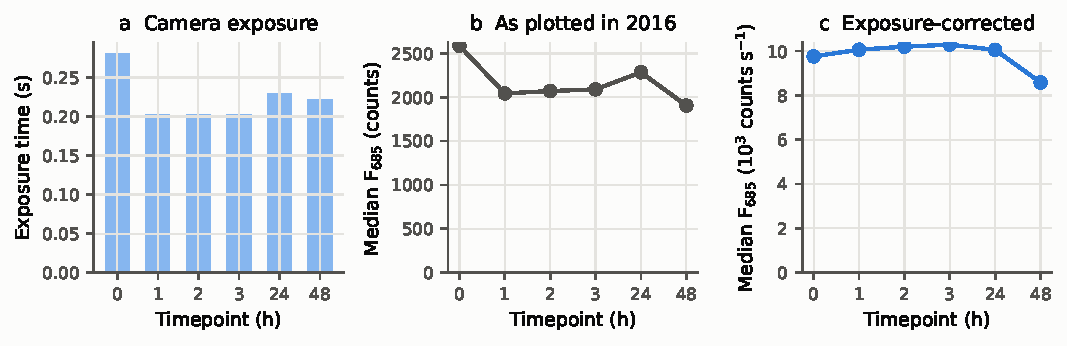
\includegraphics[width=\linewidth]{fig1_exposure_artefact.pdf}\\[2mm]
  \small The 2016 graphs' \rawDropPct{}\% intensity fall after treatment is a camera setting:
  after dividing by exposure, 1--3\,h Control values lie within \cpsDiffPct{}\% of hour 0.
\end{frame}

\begin{frame}{Data problem 2: plates differed \emph{before} treatment}
  \centering
  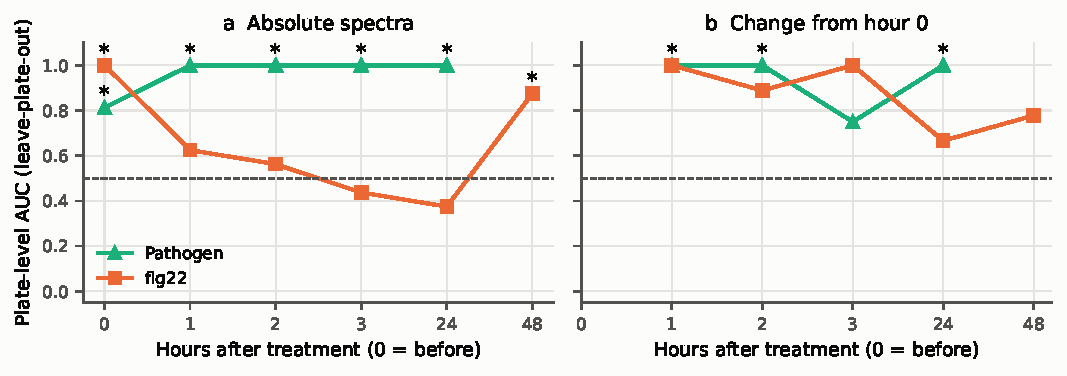
\includegraphics[width=0.85\linewidth]{fig4_auc.pdf}\\[1mm]
  \small (a) At hour 0, before any treatment, flg22 and Control plates are perfectly separable
  (AUC \aucPlaceboFlg{}). Only change from each plate's own baseline is evidence (b).
\end{frame}

\begin{frame}{Data problem 3: some 2016 exports kept the dark level}
  \begin{itemize}
    \item \nOffsetRoi{} hand-drawn spectra (all on Pathogen plates, 3\,h and 24\,h) were saved
          without dark subtraction: a flat \offsetMedian{}-count offset
    \item Uncorrected, it looks like broad ``autofluorescence'' below 640\,nm
    \item Nothing fluoresces below the 488\,nm excitation, so each spectrum's 420--470\,nm mean is
          its own offset: subtracted before any analysis
  \end{itemize}
\end{frame}

\begin{frame}{A pathogen signature from 1 hour}
  \centering
  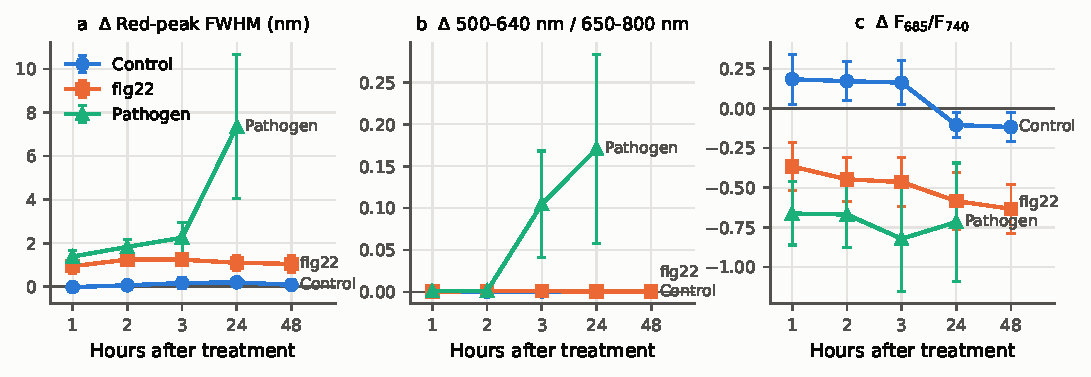
\includegraphics[width=\linewidth]{fig3_timecourse.pdf}\\[1mm]
  \small Red emission peak broadens from 1\,h (+\pathFwhmOnenm{}\,nm, $q=\pathFwhmOneq$) to 24\,h
  (+\pathFwhmTwentyFournm{}\,nm); emission below 640\,nm rises from 2\,h ($q=\pathSwTwoq$).
  At 24\,h the rise is smaller in \textit{cml24-4} ($q=\cmlFourSwq$).
\end{frame}

\begin{frame}{What the spectrum change looks like}
  \centering
  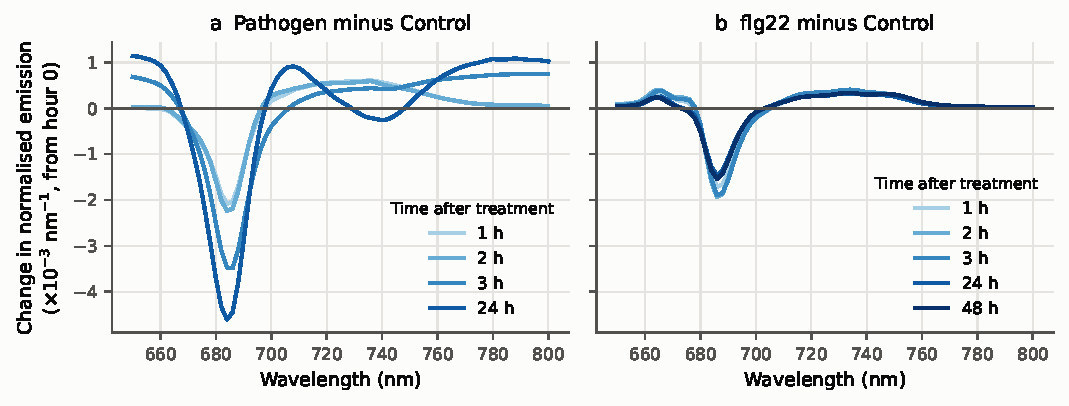
\includegraphics[width=\linewidth]{fig2_spectral_change.pdf}\\[1mm]
  \small Area-normalised spectra, change from hour 0, treated minus Control (Col-0).
\end{frame}

\begin{frame}{Infected plates can be told apart from their spectra}
  \begin{itemize}
    \item Leave-one-plate-out classifier, change-from-baseline spectra (Col-0)
    \item Plate-level AUC \aucPathOne{} at 1\,h, \aucPathTwo{} at 2\,h,
          \aucPathTwentyFour{} at 24\,h
    \item Exact permutation test over all 70 plate relabellings: $p=\pPathTwo$
    \item Weaker at 3\,h (AUC \aucPathThree, $p=\pPathThree$)
  \end{itemize}
\end{frame}

\begin{frame}{The flg22 signal is not FLS2-dependent}
  \centering
  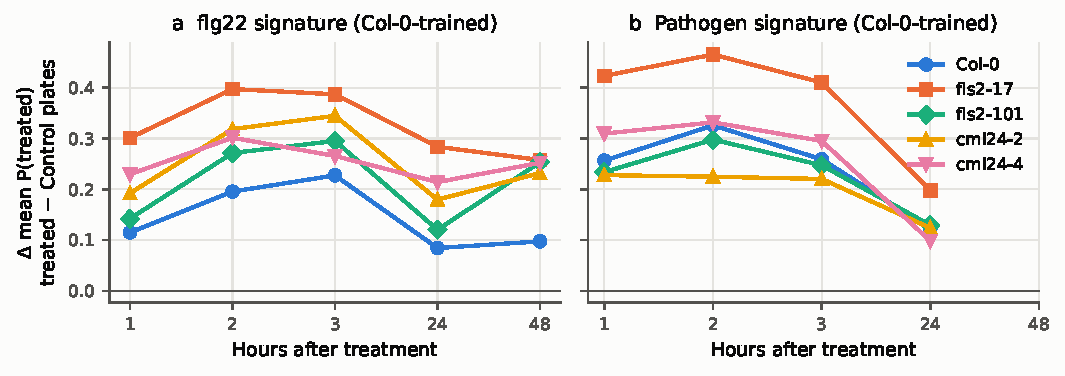
\includegraphics[width=\linewidth]{fig5_specificity.pdf}\\[1mm]
  \small A Col-0-trained flg22 model fires as strongly in \textit{fls2-17}
  (\specFlgFlsSeventeen) and \textit{fls2-101} (\specFlgFlsOneOhOne) as in Col-0
  (\specFlgColO): a plate-level effect, not perception. The pathogen signature is in every
  genotype, as expected.
\end{frame}

\begin{frame}{The November replicate}
  \begin{itemize}
    \item 405\,nm excitation; Col-0, \textit{fls2-17}, \textit{fls2-101}; 0, 6, 24, 48\,h
    \item Hand-drawn ROIs exist for only one plate per treatment, so treatment effects are
          confounded with plate there
    \item Within plates: flg22 shifts Col-0 emission shape differently from
          \textit{fls2-17} at 6\,h ($q=\setBinterq$), the FLS2-dependent pattern
    \item Raw cubes (2--3 plates/treatment): no replicated treatment effect; one deteriorating
          Control plate had the largest short-wavelength rise
    \item Bacteria-only scans do not fluoresce: the signal is the plant's
  \end{itemize}
\end{frame}

\begin{frame}{Every seedling in the raw cubes}
  \centering
  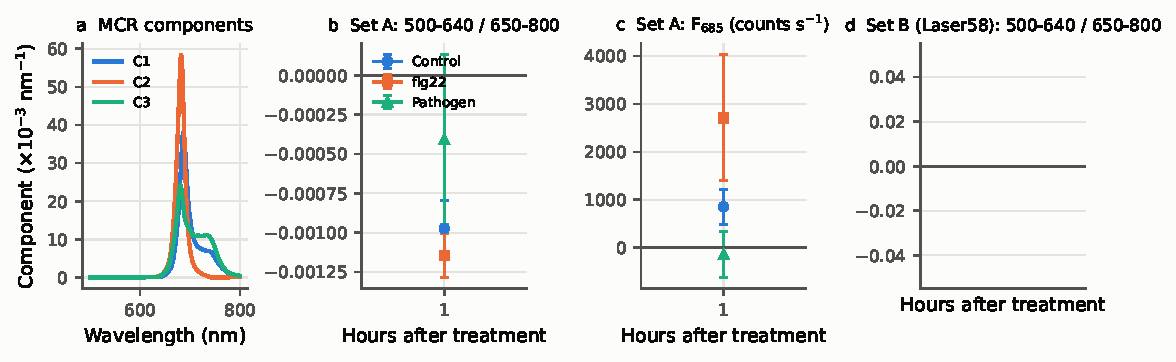
\includegraphics[width=\linewidth]{fig6_seedling_level.pdf}\\[1mm]
  \small \nSeedA{} seedlings, plate means, change from hour 0. The early signature replicates;
  685\,nm emission falls from 3\,h (\pathSeedCpsFortyEight{}\,s$^{-1}$ by 48\,h) and seedlings
  shrink. Curve resolution finds no separate broad autofluorescence component.
\end{frame}

\begin{frame}{Take-home}
  \begin{enumerate}
    \item Carry acquisition metadata with every intensity: one camera setting made the most
          striking 2016 pattern.
    \item The plate is the experimental unit: image a baseline and validate leave-plate-out.
    \item Use non-perceiving mutants as the decisive control.
    \item Check every export: an un-subtracted dark level mimicked autofluorescence.
    \item A pathogen signature appears from 1\,h (broader red peak), then chlorophyll emission
          falls and tissue is lost; short-wavelength emission marks damage, not infection.
    \item No robust CML24 effect.
  \end{enumerate}
\end{frame}

\begin{frame}{FAIR resource}
  \begin{itemize}
    \item Code, manifests, hand-ROI spectra, derived tables: \texttt{github.com/dr-richard-barker/PathoFluor-At}
    \item Raw cubes (lossless, SHA-256 verified): Zenodo \pending{DOIs}
    \item Project page: \texttt{dr-richard-barker.github.io/PathoFluor-At}
    \item Every number in the paper and these slides is generated from the committed tables
  \end{itemize}
\end{frame}

\end{document}
